\chapter{Normale Betriebsverfahren}
\pagecolor{white}
\section{Einführung}
Der vorliegende Abschnitt stellt eine Checkliste zur Verfügung und beinhaltet die Beschreibung der normalen Betriebsverfahren.

\section{Montageverfahren}
Die B13 lässt sich mit Hilfe einer Flächenstütze durch vier Personen auf- und abrüsten.

\subsection{Aufrüsten}
Das Aufrüsten der B13 geschieht in folgender Reihenfolge.\\
\newline
\underline{Vorbereitungen}
\begin{itemize}
\item Transportanhänger sichern
\item alle Bolzen und Buchsen säubern und fetten
\item Trimmung kopflastig stellen, Wölbklappen auf Stellung 0 bringen und Bremsklappen entriegeln
\item Batterie in Halterung einbauen und anschließen
\item Gepäckfach einbauen

\end{itemize}

\underline{Innenflächen}
\begin{itemize}
\item Linken Hauptbolzen in das Auge des linken Innenflügels stecken
\item Linken Holmstummel bis zur Hälfte einführen
\item Rechten Hauptbolzen in das vorgesehene Auge stecken
\item Linke Innenfläche in den Rumpf stecken und beide Hauptbolzen bis zum Querkraftrohr herausziehen
\item Rechten Innenflügel in den Rumpf stecken
\item Hauptbolzenachsen zum Fluchten bringen (dies ist nur möglich, wenn beide Flügel bis an den Rumpf eingeführt sind), Hauptbolzen eindrücken und sichern. Graue Markierung auf rechten Holmstummel kann bei der Ausrichtung der Flügel helfen. (untere Kante parallel zu Holmstummeloberkante)
\item Steuerung im Rumpf anschließen und sichern - \begin{color}{red} 2x3 Anschlüsse. (L'Hotellier) \end{color} Es kann hilfreich sein, die Querruderanschlüsse im Rumpf erst nach Montage der Außenflächen anzuschließen.
\item Sicherungsschraube am Rechten Hauptbolzen lässt sich am besten einführen, wenn Hauptbolzengriff nach unten steht, danach Hauptbolzen in vorgesehene Sicherung einrasten und Sicherungsschraube mit Fokkernadel sichern.
\end{itemize}

\underline{Außenflächen}
\begin{itemize}
\item Außenflächenbolzen-Tool in das vorgesehene Loch des Außenflächenbolzens einführen
\item Außenfläche bis auf $10cm$ in die Innenfläche einführen
\item Querruder anschließen und sichern \begin{color}{red} (L'Hotellier) \end{color}
\item Außenfläche vollständig einführen
\item Außenflächenbolzen von vorne in die Bohrung einführen
\item Außenflächenbolzen-Tool entfernen und mit dem federbelasteten Sicherungsstift die Außenflächen-Bolzen sichern 
\end{itemize}

\underline{Höhenleitwerk}
\begin{itemize}
\item M3-Montageschraube mit roter Kugel in den vorderen Anschlussbolzen an der oberen Seitenflossen-Vorderkante einschrauben
\item Höhenleitwerk auf beide Antriebsbolzen aufstecken und ganz nach hinten schieben
\item Montageschraube ziehen, das Leitwerk senkt sich ab und wird vom vorderen Anschlussbolzen gesichert, in dem die Montageschraube wieder losgelassen wird
\item Montageschraube herausschrauben (nach Herausschrauben, darf der Bolzen nicht mehr aus der Vorderkanten-Kontur der Seitenflosse herausstehen), Gewindeöffnung abkleben
\end{itemize}

\underline{Nachbereitungen}
\begin{itemize}
\item Düse in die Düsenaufname der Seitenflosse schieben
\item Antennenkabel an der Haube anschließen
\item Querruder, Wölbklappen, Bremsklappen, Höhenruder, Seitenruder auf Sicherung, Funktion und Freigängigkeit überprüfen
%\item Batterie in der vorgesehenen Halterung (hinter dem rechten Piloten) befestigen
\item Alle Trennstellen (Innenfläche-Außenfläche, Rumpf-Innenfläche, Seitenleitwerk-Höhenleitwerk) mit Isolierband abkleben
\end{itemize}
\begin{color}{red}
\large{\underline{Warnung}}\\
Bei den Ruderanschlüssen handelt es sich um manuelle Anschlüsse (L'Hotellier). Sie sind zu sichern (Federstecker) und vor jedem Flugbetrieb auf richtigen Anschluss und Sicherung zu kontrollieren!
\end{color}\\

\subsection{Abrüsten}
Das Abrüsten geht in umgekehrter Reihenfolge wie das Aufrüsten vonstatten.

\section{Tägliche Kontrolle}
Vor Beginn des Flugbetriebs muss die B13 anhand der folgenden Checkliste sorgfältig überprüft werden. Insbesondere für die Ruderproben empfiehlt sich die Unterstützung durch eine zweite Person.\\
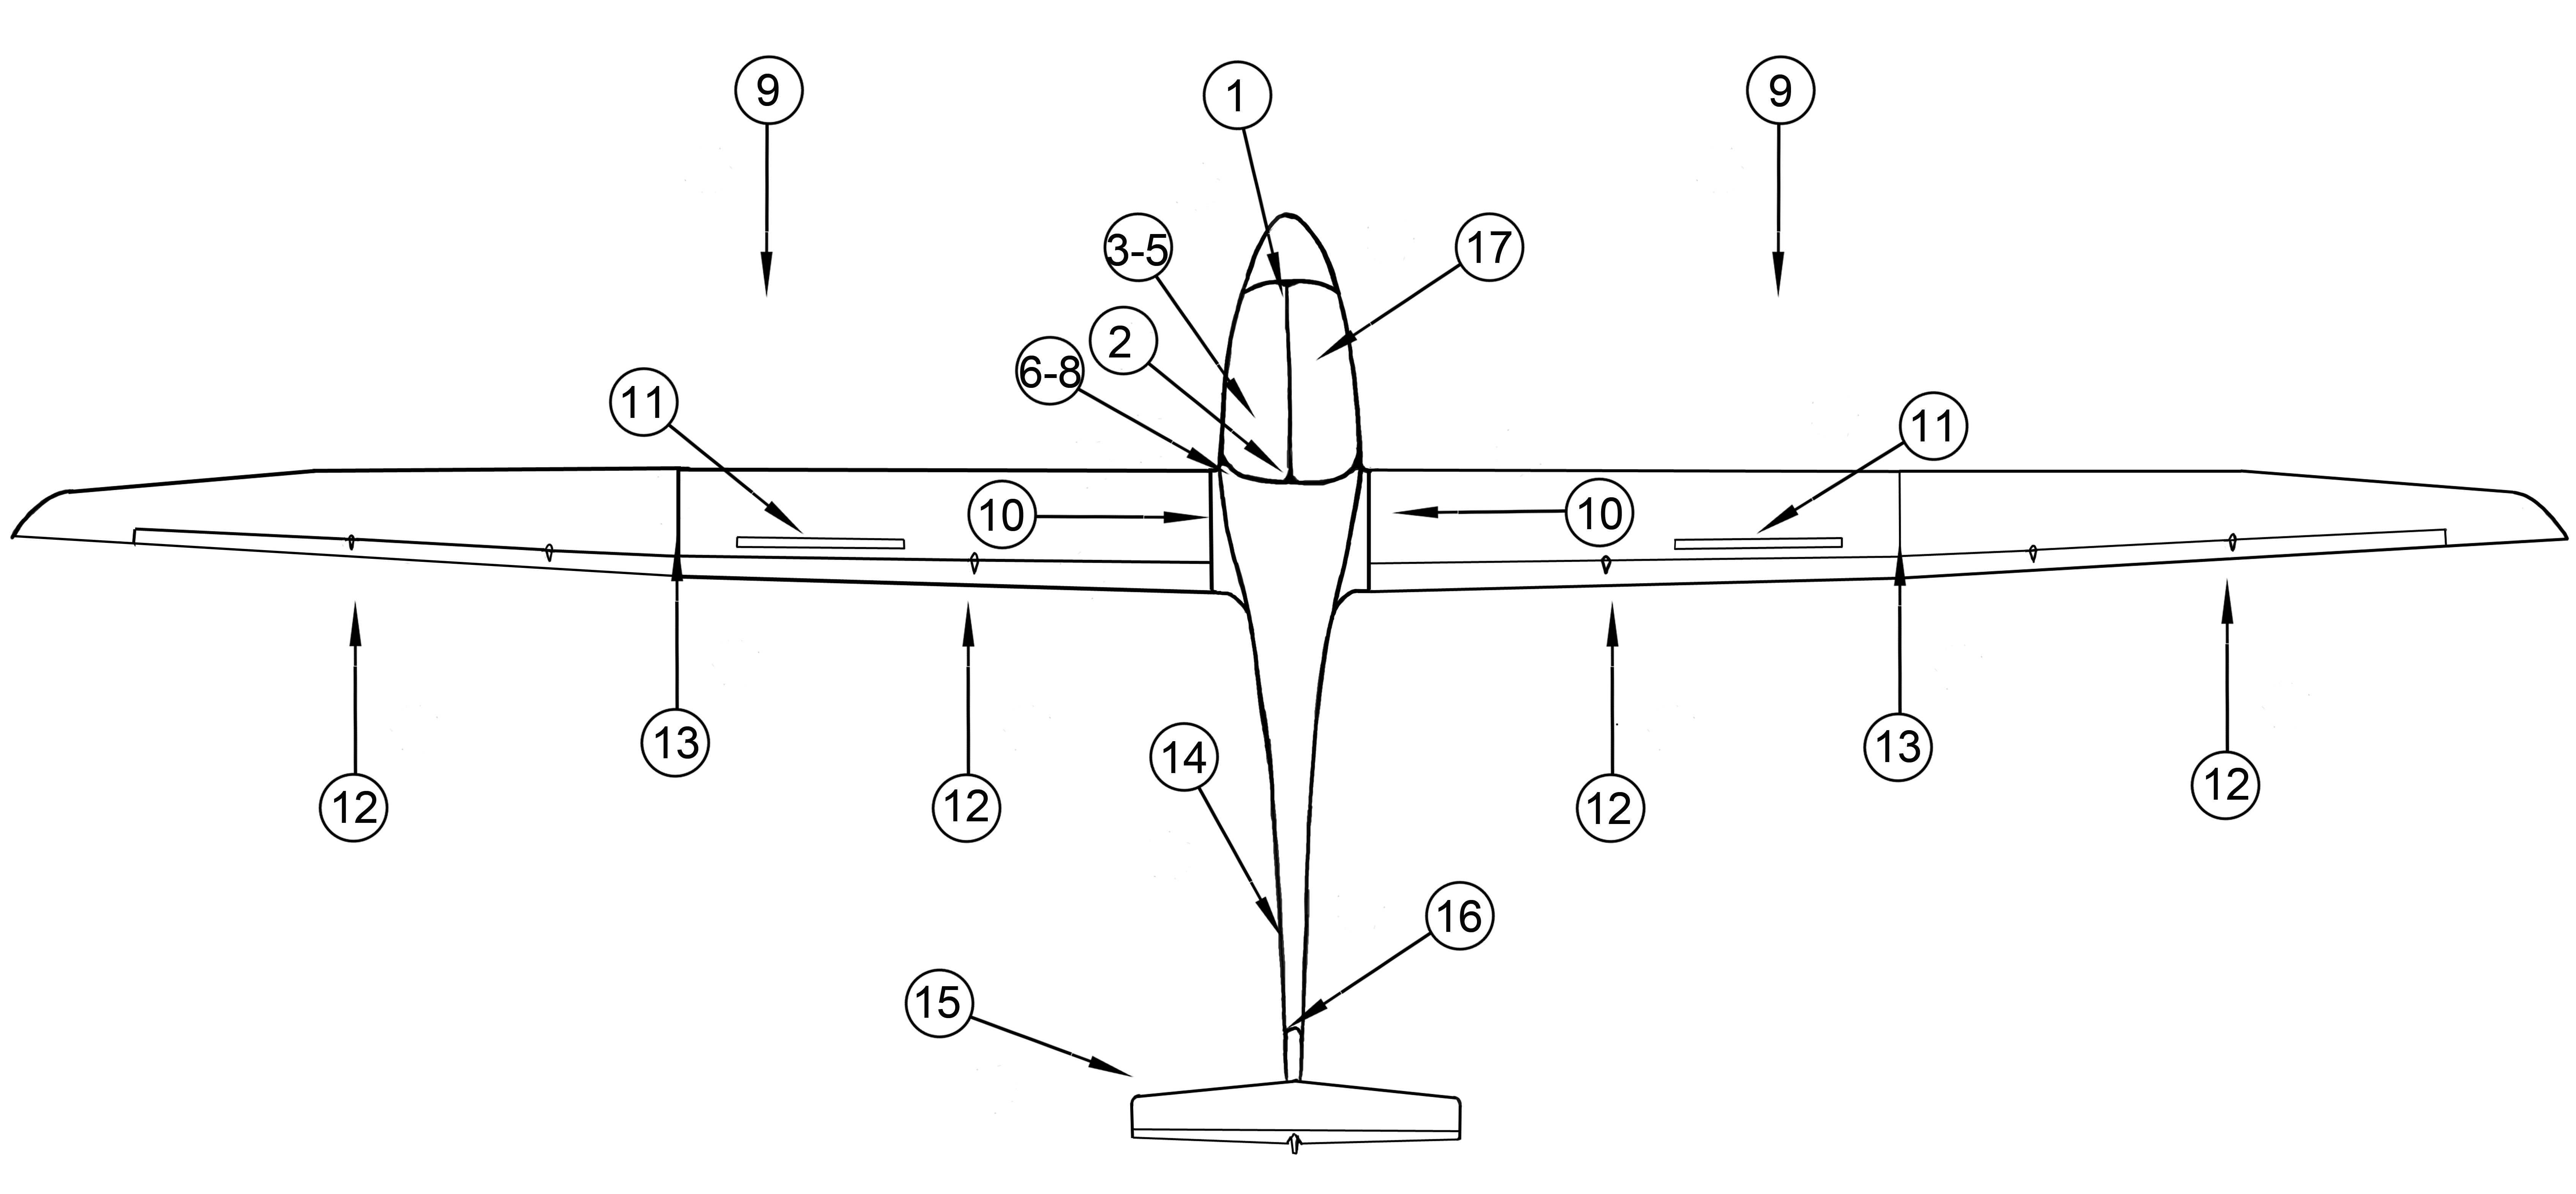
\includegraphics[width=\textwidth]{b13check.png}
\begin{enumerate}
\item Haube öffnen und Haubennotabwurf überprüfen
\item Sicherung der Hauptbolzen überprüfen
\item Fremdkörperkontrolle im gesamten Cockpitbereich
\item Freigängigkeit und Spielfreiheit aller Bedienelemente prüfen
\item Ruderprobe bei allen Rudern (Quer-, Seiten- und Höhenruder) und Klappen (Wölb- und Bremsklappe) unter Belastung durchführen und Sicherungen der Steuerung soweit einsehbar und erreichbar, überprüfen
\item Ausklinkprobe der Schleppkupplung, auch unter Last
\item Fahrwerk und Reifen auf Beschädigungen überprüfen, Luftdruck im Reifen prüfen (auch Spornrad), Rutschmarke
\item Radbremse auf Funktion und Dichtigkeit überprüfen, Abnutzungsgrad der Bremsbeläge prüfen
\item Flügelober- und Unterseite auf Beschädigungen (Lackrisse, o.ä.) überprüfen, besonders im Bereich der Flügelwurzel
\item Flügelanschlüsse auf besonderes Spiel in den Querkraftlagern prüfen
\item Bremsklappen auf Funktion, vollständiges Schließen der Abdeckungen, Fremdkörper oder Feuchtigkeit in den Kästen überprüfen
\item Flügelklappen und Anlenkungen überprüfen (Freigängigkeit, Spielfreiheit)
\item Außenflügelanschluss - Verriegelung und Sicherung überprüfen
\item Rumpfunterseite und Leitwerksträger auf Schäden (Lackrisse, etc.) 	überprüfen, besonders im Bereich der Leitwerksanschäftung (Kuller entfernen)
\item Seiten- und Höhenleitwerk auf richtige Montage, Spiel und Beschädigungen 	überprüfen, Seilzüge des Seitenruders prüfen
\item Druckabnahmen in der Seitenflosse (Dreifachdüse) überprüfen (mit 	Fahrtmesser und Variometer)
\item Elektrisches System (Funk, Rechner) überprüfen, 	Funkprobe
\end{enumerate}

\section{Vorflugkontrolle}
Die folgende Checkliste ist im Cockpit für beide Piloten gut sichtbar angebracht. Anhand ihrer ist vor jedem Start eine Vorflugkontrolle durchzuführen:
\begin{center}
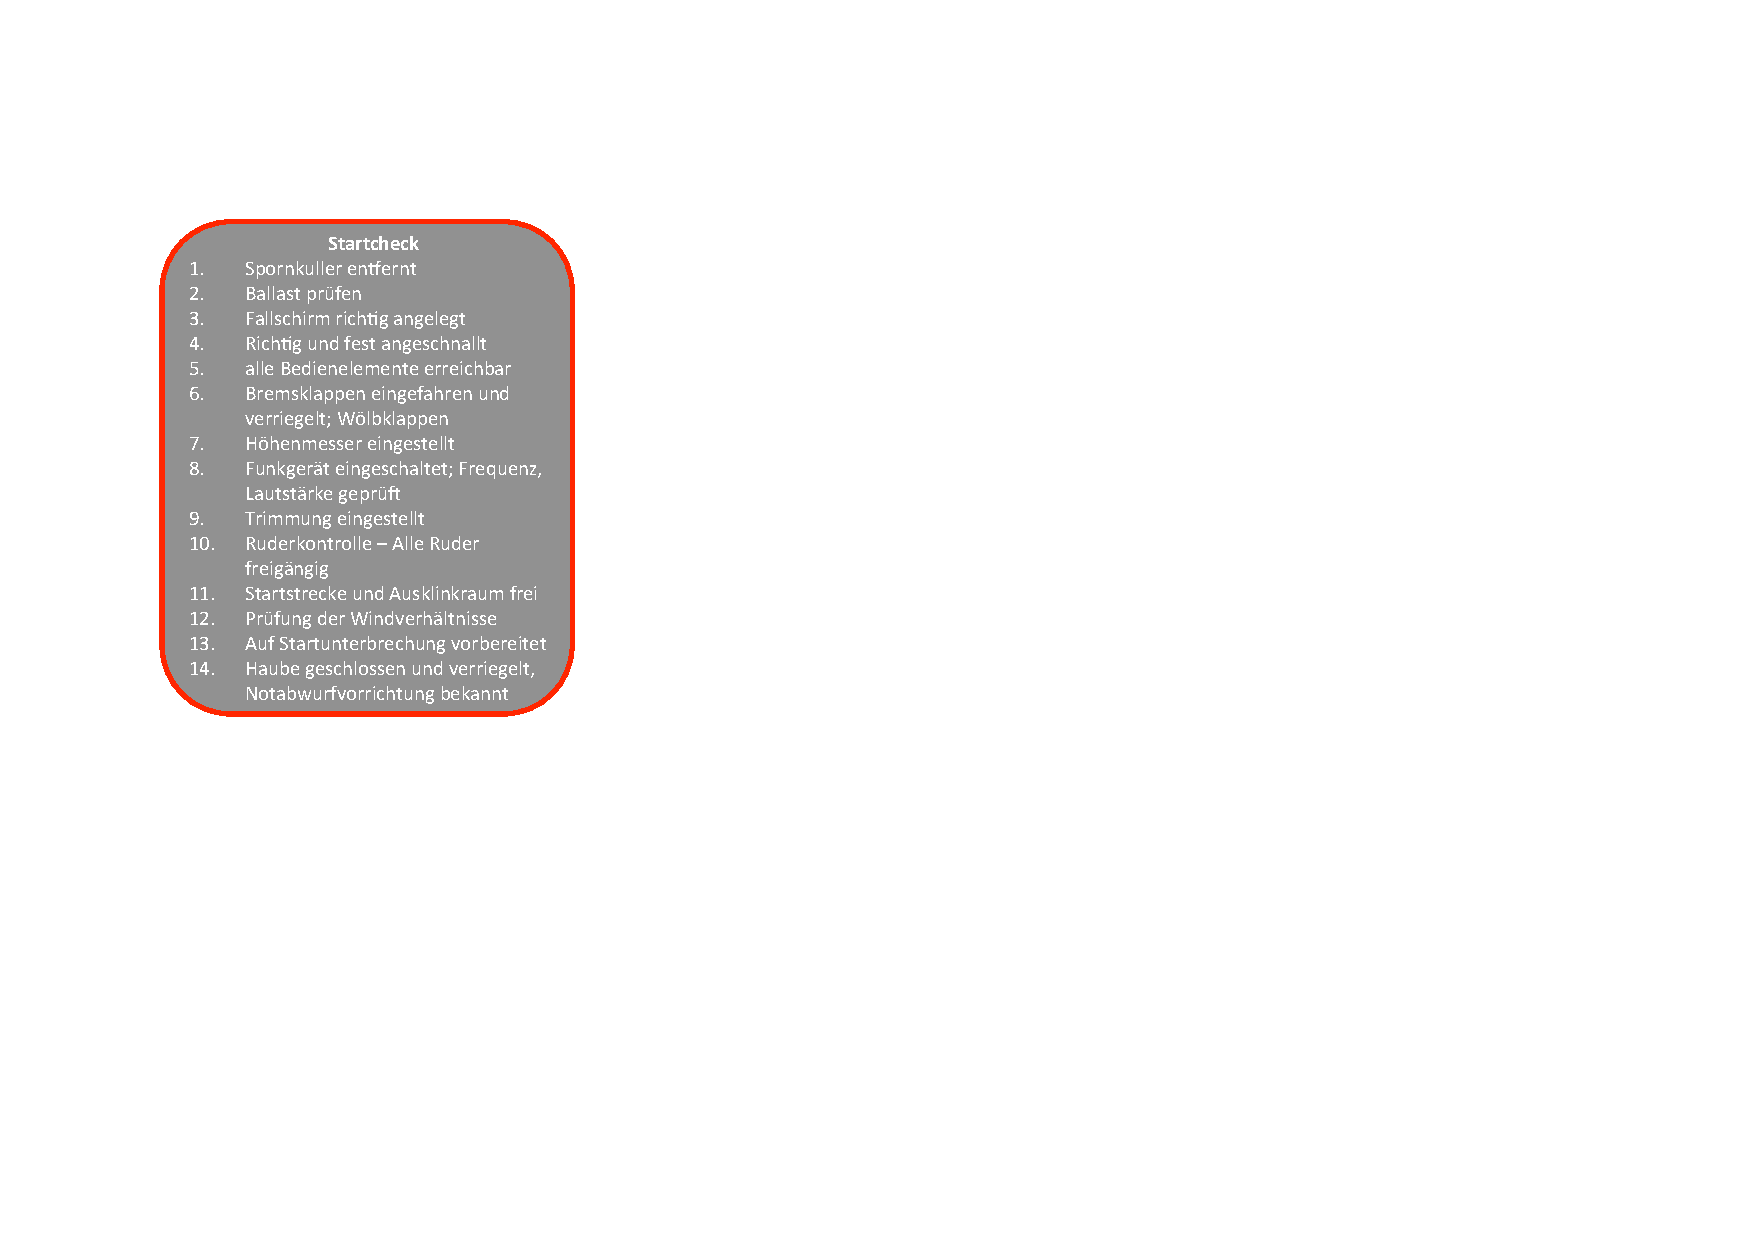
\includegraphics[width=.45\textwidth]{bilder/startcheck.pdf}
\end{center}
\section{Normalverfahren und empfohlene Geschwindigkeiten}
\subsection{Windenstart}
Die höchstzulässige Geschwindigkeit im Windenschlepp beträgt $V_W=120 \frac{km}{h}$. Die normale Schleppgeschwindigkeit beträgt $110 \frac{km}{h}$ (bei maximaler Abflugmasse $120 \frac{km}{h}$) und sollte nicht um mehr als $10 \frac{km}{h}$ unterschritten werden.\\
Vor dem Start ist die Trimmung neutral bis leicht kopflastig zu stellen. Beim Anrollen wird bis zum Erreichen von ausreichend Querruderwirkung die Wölbklappenstellung $-2$ empfohlen, danach sollte auf die Wölbklappenstellung $+1$ umgewölbt werden.\\
Das Windenseil sollte mit einer Sollbruchstelle ausgestattet sein, die eine maximalen Bruchlast von $1000 daN (schwarz)$ erreicht. \\
\newline
\begin{color}{red}
\large{\underline{Warnung}}\\
Von \underline{Rückenwindschlepps} an schwachen Schleppwinden, besonders in Zusammenhang mit hohen Außentemperaturen wird ausdrücklich abgeraten.
\end{color}\\
\newline
\begin{color}{forestgreen}
\large{\underline{Wichtiger Hinweis}}\\
Vor dem Start müssen beide Piloten ihre Sitzposition und die Erreichbarkeit der 	Bedienelemente überprüfen. Die Sitzposition, besonders mit einem Sitzkissen, muss so sein, dass ein Zurückrutschen beim Anschleppen oder im steilen Steigflug ausgeschlossen ist. Ebenso ist das sichere Einrasten der Pedalverstellungen zu 	überprüfen.
\end{color}\\
\newline
\begin{color}{forestgreen}
\large{\underline{Wichtiger Hinweis}}\\
Querneigung beachten!
\end{color}\\
\subsection{Flugzeugschlepp}
Die höchstzulässige Schleppgeschwindigkeit beträgt $V_T=160 \frac{km}{h}$. Die normale Schleppgeschwindigkeit liegt bei $110-130 \frac{km}{h}$. \\
Auch für den Flugzeugschlepp wird die Schwerpunktkupplung auf der Rumpfunterseite verwendet. Es sollte daher ein ausreichender Übungsstand bei F-Schlepps an Schwerpunktkupplungen vorliegen. Das Schleppseil sollte eine Bruchlast von $1000 daN (schwarz)$ erreichen und eine Länge zwischen $30m$ und $60m$ haben.\\
Vor dem Start ist die Trimmung in Neutralstellung zu bringen. Die Wölbklappen befinden sich in der Stellung $-2$. Sobald ausrechend Querruderwirkung vorhanden ist, wird vorsichtig auf $+1$ umgewölbt. Das Abheben erfolgt in dieser Wölbklappenstellung. \\
Bei Überlandschlepps und höheren Schleppgeschwindigkeiten kann auch auf die $0$ oder  $-1$ Stellung umgewölbt werden.\\
Das Fahrwerk kann während des Flugzeugschlepps in sicherer Höhe vorzugsweise vom Copiloten eingefahren werden.\\
\newline
\begin{color}{red}
\large{\underline{Warnung}}\\
Nicht das Schleppflugzeug übersteigen!
\end{color}\\
\newline
\begin{color}{forestgreen}
\large{\underline{Wichtiger Hinweis}}\\
Es wird empfohlen ein längeres Schleppseil aufgrund der außermittigen Sitzposition zu verwenden, um Schiebeflugzustände im F-Schlepp zu 	vermeiden. Jeder Sitz sollte zusätzlich mit einem eigenen Haubenfaden ausgestattet sein. Bei negativen Wölbklappenstellungen kann das Schleppflugzeug schnell unter dem Haubenrahmen verschwinden.
\end{color}\\
\newline
\begin{color}{forestgreen}
\large{\underline{Wichtiger Hinweis}}\\
Querneigung beachten!
\end{color}\\
\newline
\begin{color}{blue}
\large{\underline{Anmerkung}}\\
Es empfiehlt sich, vor dem Anrollen die Radbremse leicht anzuziehen, damit ein	Überrollen des Schleppseils vermieden wird. 
\end{color}\\
\begin{color}{blue}
\large{\underline{Anmerkung}}\\
Die Schleppmaschine sollte aufgrund des hohen Abfluggewichtes der B13 ausreichend motorisiert sein.
\end{color}\\

\subsection{Freier Flug}
Die B13 zeigt bei allen Schwerpunktlagen, Beladungszuständen, Wölbklappenstellungen und Fluggeschwindigkeiten ein angenehmes Flugverhalten. Unangenehme Eigenschaften wurden bisher nicht ermittelt. Im freien Geradeausflug kann man alle Ruder freigeben, ohne daß das Flugzeug dazu neigt eine neue Fluglage einzunehmen. Um einen schiebefreien Flug zu erreichen, sollte jeder Sitz über einen eigenen Faden verfügen.\\
\newline
Der Trimmbereich geht von ca. $80 \frac{km}{h}$ bis zu über $220 \frac{km}{h}$. Die Kurvenwechselzeiten aus $45^{\circ}$ - Kurven liegen bei ungefähr $4s$.\\

\begin{itemize}
\item \textbf{Gebrauch der Wölbklappen}\\
Die optimale Stellung der Wölbklappen hängt stark von der Flächenbelastung ab. Für eine Flächenbelastung von $\frac{G}{S}=396 \frac{N}{m^2}$ sind die Geschwindigkeits- und Gleitzahlpolare in Kapitel 5.3.2 und 5.3.3 abgebildet. 
Es sollte darauf geachtet werden, daß ein ruckartiges Betätigen der Wölbklappen eventuell ein Durchsacken oder Wegsteigen bewirken könnte. Dieses Verhalten kann besonders in Bodennähe zu kritisch Situationen führen. Die Wölbklappen sollten daher immer langsam und kontinuierlich betätigt werden. 
\item \textbf{Überzieheigenschaften}\\
Der überzogene Flugzustand äußert sich bei der B13 durch weiche Ruder, Taumeln, Nicken, Schütteln und schließlich dem Sackflug. Bei diesen hohen Anstellwinkeln muss davon ausgegangen werden, dass die Fahrtmesseranzeige stark durch die Strömungsablösungen am Rumpf beeinflusst wird und daher keine richtigen Fluggeschwindigkeiten anzeigt.  Der überzogene Flugzustand oder gar ein Abkippen über eine Fläche kann durch Nachlassen des Höhensteuers und – wenn erforderlich – durch Gegenseitenruder beendet werden. 
\item \textbf{Schnellflug}\\
Für den Schnellflug sind die Klappenstellungen $0$, $-1$ und $-2$ vorgesehen. Es sollte darauf geachtet werden, dass die $V_{NE} = 220 \frac{km}{h}$  und die maximalen Abfanglastvielfachen nicht überschritten werden. Weiterhin dürfen ab der Manövergeschwindigkeit von $V_A = 160 \frac{km}{h}$ nur noch $\frac{1}{3}$ der Ruderausschläge gegeben werden. 

\end{itemize}
\newpage
\subsection{Benutzen des Triebwerks während des Fluges}
nicht eingebaut
\newpage
\subsection{Landeanflug}
An dem Punkt "`Position"' wird folgende Lande-Checkliste durchgeführt:
\newline
\begin{center}
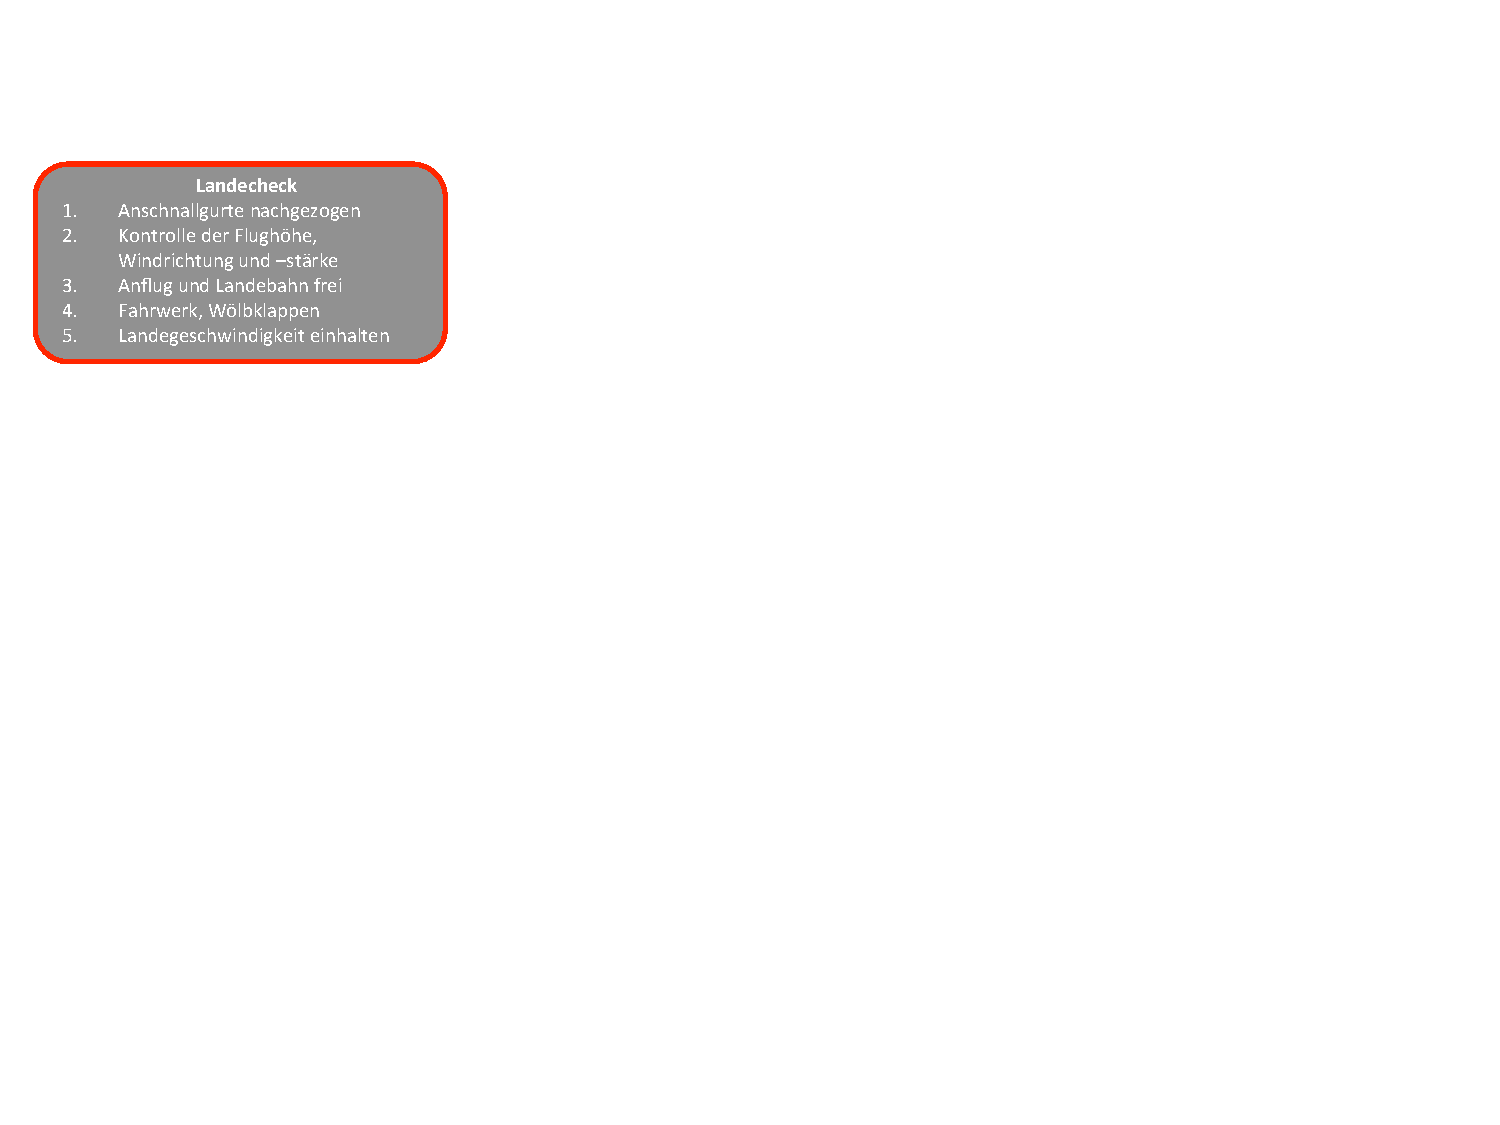
\includegraphics[width=.45\textwidth]{bilder/landecheck.pdf}
\end{center}


Die normale Anfluggeschwindigkeit für die maximale Masse mit voll ausgefahrenen Bremsklappen und ausgefahrenen Fahrwerk liegt bei $100 \frac{km}{h}$ (gelbes Dreieck auf dem Fahrtmesser).\\
Die Wirkung eines Seitengleitfluges und der doppelstöckigen Schempp-Hirth-Bremsklappen ist gering. (Gleitzahl bei ausgefahrenen Bremsklappen ca. $9,2$) \\
Für kurze Landungen über ein Hindernis wird es erfahrenen Piloten empfohlen, schon in größerer Höhe die Fahrt zu reduzieren, da die Wirkung des Bodeneffektes beachtlich ist.\\
Die B13 sollte mit voll gezogenem Höhenruder in 2-Punkt-Lage aufgesetzt werden, Spornradlandungen sind auch problemlos möglich. Nach dem Aufsetzen sollte auf die Wölbklappenstellung $-2$ umgewölbt werden, um die Querruderwirkung bis zum Stillstand aufrecht zu erhalten. Es empfiehlt sich, den Copiloten dabei die Bremsklappen in der gewünschten Stellung festhalten zu lassen, um ein hereinfallen dieser zu verhindern. \\
Die Radbremse wird bei vollem ausfahren der Bremsklappen mitbetätigt und ist gut wirksam.
Das Fahrwerk muss immer ausgefahren werden, da es den Piloten und die Flugzeugstruktur vor starken Landestößen schützt.\\
\newline
\begin{color}{blue}
\large{\underline{Anmerkung}}\\
Aufgrund der Sitzposition sollte die Platzrunde in Richtung des fliegenden Luftfahrzeugführers bevorzugt werden, da die Sichtverhältnisse zur anderen Seite eingeschränkt sind.
\end{color}\\
\newline
\begin{color}{forestgreen}
\large{\underline{Wichtiger Hinweis}}\\
Der Seitengleitflug ist nur wenig wirksam und deshalb als Landehilfe nur bedingt geeignet.
\end{color}\\
